%%%%%%%%%%%%%%%%%%%%%%%%%%%%%%%%%%%%%%%%%%%%%%%%%%%%%%%%%%%%%%%%%%%%%%%%%%%%%%%%
\section{Getting Started with Snakemake}

%%%%%%%%%%%%%%%%%%%%%%%%%%%%%%%%%%%%%%%%%%%%%%%%%%%%%%%%%%%%%%%%%%%%%%%%%%%%%%%%
\subsection{Goals, Background \& Outline}

%%%%%%%%%%%%%%%%%%%%%%%%%%%%%%%%%%%%%%%%%%%%%%%%%%%%%%%%%%%%%%%%%%%%%%%%%%%%%%%%
\begin{frame}
  \frametitle{Questions}
  \question[The questions you most probably have when starting your Analysis:]{\begin{itemize}
                                                                               \item How to start quickly (with the lowest amount of overhead)?
                                                                               \item What are the necessary tools?
                                                                               \end{itemize}}
                                                                               
  \question[My question to you:]{How do you get this information? And: Is reproducibility and sustainability your concern?}
  \pause
  \begin{block}{Most frequent answers}
   \begin{itemize}
    \item Your labmate(s)
    \item The Internet
    \item Yes, of course ... eventually, when I write my paper/thesis.
   \end{itemize}
  \end{block}
\end{frame}

%%%%%%%%%%%%%%%%%%%%%%%%%%%%%%%%%%%%%%%%%%%%%%%%%%%%%%%%%%%%%%%%%%%%%%%%%%%%%%%%
\begin{frame}
  \frametitle{The Workflow Approach}
  Workflow Engines answer these questions directly by providing
  \begin{itemize}
   \item Entire Workflows can be selected and can be put to action.
   \item The do the same thing always (and take care of other aspects of reproducibility, like to protocol parameters).
  \end{itemize}
\end{frame}

%%%%%%%%%%%%%%%%%%%%%%%%%%%%%%%%%%%%%%%%%%%%%%%%%%%%%%%%%%%%%%%%%%%%%%%%%%%%%%%%
\begin{frame}
  \frametitle{Going HPC}
  \question{Why would you want to work on a cluster?}
  \pause
  Answers may include:
  \begin{itemize}[<+->]
   \item a curated workflow repository containing
   \item configurable workflows.
  \end{itemize}
\end{frame}

%%%%%%%%%%%%%%%%%%%%%%%%%%%%%%%%%%%%%%%%%%%%%%%%%%%%%%%%%%%%%%%%%%%%%%%%%%%%%%%%
\begin{frame}
  \frametitle{Why \emph{Snakemake} 
\includegraphics[width=2em]{logos/Snakemake.png}?}
  \begin{columns}
    \begin{column}{0.5\textwidth}
      \begin{itemize}[<+->]
   \item extremely feature rich
   \item over 1800 workflows in \lhref{https://snakemake.github.io/snakemake-workflow-catalog/}{its catalogue}
   \item almost a hundred standardized (meaning: will documented and with automatic deployment)
   \item cluster batch systems are supported (and support for various cloud systems, too)
   \item there is an option to include Nextflow wrappers, too.
      \end{itemize}
    \end{column}
    \begin{column}{0.5\textwidth}
      \begin{figure}
        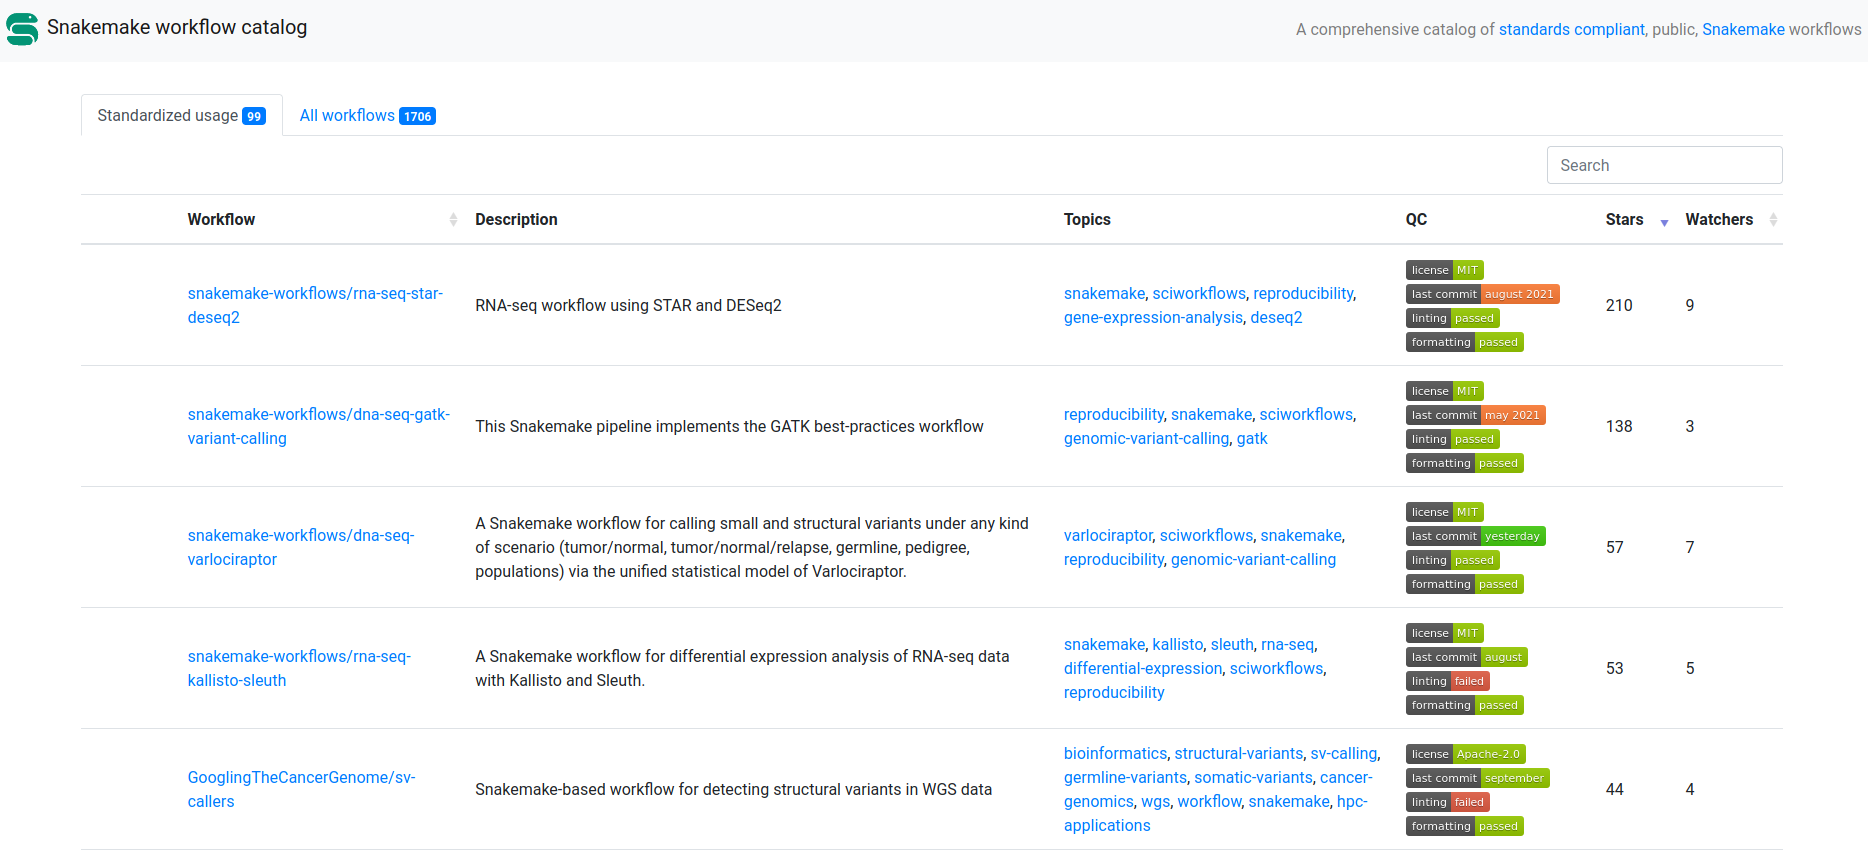
\includegraphics[width=\textwidth]{Snakemake/Snakemake_Workflow_Catalog.png}
        \caption{Screenshot of the Workflow Catalogue}
      \end{figure}
    \end{column}
  \end{columns}
\end{frame}

%%%%%%%%%%%%%%%%%%%%%%%%%%%%%%%%%%%%%%%%%%%%%%%%%%%%%%%%%%%%%%%%%%%%%%%%%%%%%%%%
\begin{frame}[fragile]
  \frametitle{The Tasksetting I}
  We give ourselves a little (proxy) task. Suppose you want to analyse the frequency of words in certain books.\newline
  \pause
  We’ve compiled our raw data i.e. the books we want to analyse and have prepared several Python scripts that together make up our analysis workflow. -- Our example directory is:
  \pathtoexercise{}\newline
  For starters we just copy the entire directory:
  \begin{lstlisting}[language=Bash, style=Shell]
$ # work in your home directory, if unsure, perform
$ cd # to go there
$ # copy the example directory
$ cp -r /lustre/project/m2_jgu-ngstraing/workflows @.@
$ # change to the workflows directory:
$ cd workflows
  \end{lstlisting}
  \hint{Use TAB-completion to get the entire path typed. Save yourself the mental effort to type!}
\end{frame}

%%%%%%%%%%%%%%%%%%%%%%%%%%%%%%%%%%%%%%%%%%%%%%%%%%%%%%%%%%%%%%%%%%%%%%%%%%%%%%%%
\begin{frame}[fragile]
  \frametitle{The Tasksetting II}
  Now, let us look, what we have here!\newline
  Using the command \texttt{head}, we can have a look in our data, e.\,g.:
  \begin{lstlisting}[language=Bash, style=Shell, basicstyle=\ttfamily\footnotesize]
$ head books/isles.txt
  \end{lstlisting}
\end{frame}

%%%%%%%%%%%%%%%%%%%%%%%%%%%%%%%%%%%%%%%%%%%%%%%%%%%%%%%%%%%%%%%%%%%%%%%%%%%%%%%%
\begin{frame}[fragile]
  \frametitle{The Tasksetting III}
  This will (per default) the first 10 lines:
  \begin{lstlisting}[style=Plain, basicstyle=\ttfamily\tiny]
A JOURNEY TO THE WESTERN ISLANDS OF SCOTLAND


INCH KEITH


I had desired to visit the Hebrides, or Western Islands of Scotland, so
long, that I scarcely remember how the wish was originally excited; and
was in the Autumn of the year 1773 induced to undertake the journey, by
finding in Mr. Boswell a companion, whose acuteness would help my
  \end{lstlisting}
  \pause
  \task{Perform the \texttt{head}-command on any other book.}
\end{frame}

%%%%%%%%%%%%%%%%%%%%%%%%%%%%%%%%%%%%%%%%%%%%%%%%%%%%%%%%%%%%%%%%%%%%%%%%%%%%%%%%
\begin{frame}[fragile]
  \frametitle{The Tasksetting IV}
  What else is there?\newline
  We can use the \texttt{tree} command to display the content of an entire directory tree, e.\,g.:
  \begin{columns}
    \begin{column}{0.2\textwidth}
    \footnotesize
     Should display something like (and more):
    \end{column}
    \begin{column}{0.8\textwidth}
    \begin{minipage}[t]{0.5\textwidth}
    \setstretch{0.1}
            {\tiny \DTsetlength{0.2em}{1em}{0.2em}{0.4pt}{.6pt}
\texttt{\$ tree}
\dirtree{%
.1 /.
.2 books.
.3 {abyss.txt}\DTcomment{a book}.
.3 {isles.txt}.
.3 {last.txt}.
.3 {sierra.txt}.
.2 zipfs\_analysis.
.3 scripts.
.4 {plotcount.py}\DTcomment{a script}.
.4 {wordcount.py}.
.4 {\ldots}.
.3 {Snakefile}\DTcomment{our workflow}.
}}
    \end{minipage}


    \end{column}
  \end{columns}
\end{frame}

%%%%%%%%%%%%%%%%%%%%%%%%%%%%%%%%%%%%%%%%%%%%%%%%%%%%%%%%%%%%%%%%%%%%%%%%%%%%%%%%
\begin{frame}[fragile]
  \frametitle{\Interlude{About Module Files}}
  On HPC Systems Software is provisioned as so-called module files. For example:
  \begin{lstlisting}[language=Bash, style=Shell]
$ module load lang/Python
  \end{lstlisting}
  will load the most recent Python module and provide you with the correct environment.
  \task{Run \texttt{python --version}, then load the module and run\newline \texttt{python --version} once more.}
\end{frame}

%%%%%%%%%%%%%%%%%%%%%%%%%%%%%%%%%%%%%%%%%%%%%%%%%%%%%%%%%%%%%%%%%%%%%%%%%%%%%%%%
\begin{frame}[fragile]
  \frametitle{About \texttt{Conda}}
  Now, on HPC-systems scientific software is a provided as module files and provisioned by ``build frameworks'' like \texttt{easybuild} or \texttt{spack}. With \texttt{snakemake} we are going to \texttt{Conda}. Why? Some pros and cons:\footnotesize
  \begin{itemize}[<+->]
   \item no build-framework provides 100\,\% coverage of all needs -- including \texttt{Conda}
   \item using \texttt{Conda} has a draw-back: software is pre-build. This means: No optimizations for particular CPUs == slower execution, higher CO$_2$ footprint!
   \item HPC applications often need MPI-bindings (this cannot be provided by \texttt{Conda})
   \item \texttt{Conda} provides an enormous amount of applications for genome oriented bioinformatics
   \item to be reproducible you sometimes need older applications (which are not included in HPC build frameworks)
   \item workflow engines (like the one we are going to use rely on \texttt{Conda} and are able to install the software \emph{for you} without further setups from you!)
  \end{itemize}
  \pause
  \hint[Info:]{Upcoming releases allow to re-compile for particular platforms and help limiting up execution times.} 
\end{frame}

\begin{frame}<handout:0>
  \frametitle{Not now \ldots}
  We will be learning about \texttt{Conda} on a cluster a little later. For now, we will be working with module files and first dive into simnple workflows.
\end{frame}

%https://waylonwalker.com/install-miniconda/

%%%%%%%%%%%%%%%%%%%%%%%%%%%%%%%%%%%%%%%%%%%%%%%%%%%%%%%%%%%%%%%%%%%%%%%%%%%%%%%%
\begin{frame}[fragile]
  \frametitle{\Interlude{About Module Files II}}
  Eventually we will need a plotting module and a numeric library, too. Please run:
  \begin{lstlisting}[language=Bash, style=Shell]
$ module purge # to get a clean environment again
$ module load vis/matplotlib
  \end{lstlisting}
  \pause
  \question{Which is your version of Python, now?}
\end{frame}

%%%%%%%%%%%%%%%%%%%%%%%%%%%%%%%%%%%%%%%%%%%%%%%%%%%%%%%%%%%%%%%%%%%%%%%%%%%%%%%%
\begin{frame}[fragile]
  \frametitle{The Tasksetting V}
  The first step is to count the words.\newline
  \begin{enumerate}
   \item run \begin{lstlisting}[language=Bash, style=Shell, basicstyle=\footnotesize] 
$ python zipfs_analysis/scripts/wordcount.py \
> -i books/isles.txt -o isles.dat           
             \end{lstlisting}
  \item be aware: the \texttt{\textbackslash} and \texttt{>} are only there to fit everything on screen
  \item take a quick look at the results:
        \begin{lstlisting}[language=Bash, style=Shell] 
head -5 isles.dat
        \end{lstlisting}
  \item this shows us the 5 top lines of the result file:
  \begin{lstlisting}[style=Plain]
the 3822 6.7371760973
of 2460 4.33632998414
and 1723 3.03719372466
to 1479 2.60708619778
a 1308 2.30565838181
  \end{lstlisting}
   \end{enumerate}
\end{frame}

%%%%%%%%%%%%%%%%%%%%%%%%%%%%%%%%%%%%%%%%%%%%%%%%%%%%%%%%%%%%%%%%%%%%%%%%%%%%%%%%
\begin{frame}[fragile]
  \frametitle{The Tasksetting VI}
  Let’s visualise the results. The script \texttt{plotcount.py} reads in a data file and plots the 10 most frequently occurring words as a text-based bar plot:
  \begin{lstlisting}[language=Bash, style=Shell] 
$ python zipf_analysis/scripts/plotcount.py \
> -i isles.dat --type ascii
  \end{lstlisting}
  \pause
  Or your can create a graphical plot:
  \begin{lstlisting}[language=Bash, style=Shell] 
$ python zipf_analysis/scripts/plotcount.py \
> -i isles.dat -o isles.png
# subsequently run
$ display isles.png
  \end{lstlisting}
\end{frame}

%%%%%%%%%%%%%%%%%%%%%%%%%%%%%%%%%%%%%%%%%%%%%%%%%%%%%%%%%%%%%%%%%%%%%%%%%%%%%%%%
\begin{frame}
  \frametitle{\Interlude{Zipf’s Law}}
  
Zipf’s Law is an empirical law formulated using mathematical statistics that refers to the fact that many types of data studied in the physical and social sciences can be approximated with a Zipfian distribution, one of a family of related discrete power law probability distributions.

Zipf’s law was originally formulated in terms of quantitative linguistics, stating that given some corpus of natural language utterances, the frequency of any word is inversely proportional to its rank in the frequency table. For example, in the Brown Corpus of American English text, the word ``the'' is the most frequently occurring word, and by itself accounts for nearly 7\% of all word occurrences (69,971 out of slightly over 1 million). True to Zipf’s Law, the second-place word of accounts for slightly over 3.5\% of words (36,411 occurrences), followed by and (28,852). Only 135 vocabulary items are needed to account for half the Corpus.

Source: \lhref{https://en.wikipedia.org/wiki/Zipf\%27s\_law}{Wikipedia}
\end{frame}

%%%%%%%%%%%%%%%%%%%%%%%%%%%%%%%%%%%%%%%%%%%%%%%%%%%%%%%%%%%%%%%%%%%%%%%%%%%%%%%%
\begin{frame}[fragile]
  \frametitle{The Tasksetting VII}
  Now, we can run our statistical analyis:
  \begin{lstlisting}[language=Bash, style=Shell]
$ python zipf_analysis/scripts/zipf_test.py isles.dat
  \end{lstlisting}
  \pause
  This means, we can put it all in a \emph{Pipeline} and do our analysis!11!!
  \begin{lstlisting}[language=Bash, style=Shell, basicstyle=\tiny]
#!/bin/bash
python zipf_analysis/scripts/wordcount.py -i books/isles.txt -o isles.dat
python zipf_analysis/scripts/wordcount.py -i books/abyss.txt -o abyss.dat

python zipf_analysis/scripts/plotcount.py -i isles.dat -o isles.png
python zipf_analysis/scripts/plotcount.py -i abyss.dat -o abyss.png

# Generate summary table
python zipf_analysis/scripts/zipf_test.py abyss.dat isles.dat @>@ results.txt
  \end{lstlisting}
  \hint{The \texttt{>} sign is a redirection in \texttt{bash}.}
\end{frame}

%%%%%%%%%%%%%%%%%%%%%%%%%%%%%%%%%%%%%%%%%%%%%%%%%%%%%%%%%%%%%%%%%%%%%%%%%%%%%%%%
\begin{frame}
  \frametitle{Summary}
  This  shell script solves several problems in computational reproducibility:
  \begin{enumerate}[<+->]
   \item It explicitly documents our pipeline, making communication with colleagues (and our future selves) more efficient.
   \item It allows us to type a single command, bash \texttt{run\_pipeline.sh}, to reproduce the full analysis.
   \item It prevents us from repeating typos or mistakes. You might not get it right the first time, but once you fix something it’ll stay fixed.
  \end{enumerate}
  \pause
  \question{What are the shortcomings of this solution?}
\end{frame}

%%%%%%%%%%%%%%%%%%%%%%%%%%%%%%%%%%%%%%%%%%%%%%%%%%%%%%%%%%%%%%%%%%%%%%%%%%%%%%%%
\begin{frame}[fragile]
  \frametitle{Conclusion}
  \begin{enumerate}[<+->]
   \item Suppose you want to change settings of the plot(s). And the compute work would take longer. A manual outcomment would be required.
   \item More inputs will require to add more line or be clever with loops, e.\,g.:
         \begin{lstlisting}[language=Bash, style=Shell]
for book in books/*txt; do 
  python scripts/wordcount.py 
         -i ${book} -o {book/txt/png}
done
         \end{lstlisting}
  \end{enumerate}
  Or something similar ...\newline
  What we \emph{really} want is an executable description of our pipeline that allows software to do the tricky part for us: figuring out what tasks need to be run where and when, then perform those tasks for us!
\end{frame}

%%%%%%%%%%%%%%%%%%%%%%%%%%%%%%%%%%%%%%%%%%%%%%%%%%%%%%%%%%%%%%%%%%%%%%%%%%%%%%%%
\begin{frame}[fragile]
  \frametitle{One last Thing}
  Please delete all previous outputs:
  \begin{lstlisting}[language=Bash, style=Shell]
rm *dat *png 
  \end{lstlisting}
  \hint{\texttt{Snakemake} will recognize existing outputs and skip processes, which would be redundant.}
\end{frame}




